\documentclass[conference]{IEEEtran}

% -----------------------------
% Packages
% -----------------------------
\usepackage{graphicx}
\usepackage{ragged2e}
\usepackage{amssymb}
\usepackage{amsmath}
\usepackage{booktabs}
\usepackage{array}
\usepackage{balance}
\usepackage[backend=bibtex,style=ieee]{biblatex}
\addbibresource{references.bib}

% -----------------------------
% Bibliography Heading
% -----------------------------
\defbibheading{bibliography}[\refname]{%
  \section{\MakeUppercase{REFERENCES}}}

% -----------------------------
% Custom Column Types
% -----------------------------
\newcolumntype{L}[1]{>{\raggedright\arraybackslash}p{#1}}
\newcolumntype{C}[1]{>{\centering\arraybackslash}p{#1}}
\newcolumntype{R}[1]{>{\raggedleft\arraybackslash}p{#1}}

% -----------------------------
% Title / Author
% -----------------------------
\title{Open-Set Qur'anic Reciter Recognition Using Hybrid Acoustic Features: A Comparative Evaluation of Random Forest and Bidirectional LSTM Models}

\author{
\IEEEauthorblockN{Abdusamii Abdulazeez\IEEEauthorrefmark{1} and Habeeb Omotunde\IEEEauthorrefmark{2}}
\IEEEauthorblockA{\IEEEauthorrefmark{1}Information Technology, Imam Mohammad Ibn Saud Islamic University, Riyadh, Saudi Arabia\\
443022312@sm.imamu.edu.sa}
\IEEEauthorblockA{\IEEEauthorrefmark{2}Information Systems, Imam Mohammad Ibn Saud Islamic University, Riyadh, Saudi Arabia\\
homotunde@imamu.edu.sa}
}

% -----------------------------
% Document Start
% -----------------------------
\begin{document}

\maketitle
\begin{abstract}
Automatic Qur'anic reciter recognition is increasingly important for digital learning and recitation verification, yet limited attention has been given to open-set scenarios involving previously unseen reciters. This paper presents Qurr\={a}, an open-set reciter recognition framework that combines hybrid acoustic features---MFCC, spectral, rhythmic, tonal, and chroma descriptors---with a reliability-based rejection mechanism. Random Forest (RF) and Bidirectional LSTM (BLSTM) classifiers are compared under surah-separated evaluation using 2,535 training recordings from five reciters and 399 external recordings from seven reciters. On closed-set external evaluation (228 recordings, unseen surahs), RF achieved 100.0\% accuracy (Macro F1: 1.000) versus 97.81\% (0.978) for BLSTM. For open-set evaluation (171 unseen reciters), RF achieved 97.66\% rejection accuracy and a 2.34\% false positive rate, compared with 87.13\% and 12.87\% for BLSTM; overall external accuracies were 95.24\% and 88.97\%, respectively. The results demonstrate that hybrid acoustic representations with classical ensemble learning remain highly effective for Qur'anic reciter recognition and open-set rejection.
\end{abstract}

\begin{IEEEkeywords}
Qur'anic reciter recognition, open-set recognition, Random Forest, bidirectional LSTM, MFCC, acoustic features, speech processing, Arabic speech recognition, machine learning, speaker identification.
\end{IEEEkeywords}

% -----------------------------
% Main Text
% -----------------------------
\section{Introduction}

The Holy Qur'an has been preserved for centuries through authenticated oral transmission and precise recitation practices. Accurate recitation plays a central role in Qur'anic learning and religious practice, motivating the development of computational systems capable of analyzing and understanding recitation audio. With the growth of digital learning platforms and artificial intelligence applications in education, there is increasing interest in automated Qur'anic audio analysis systems \cite{ref2, ref9, ref10}.

Automatic Qur'anic recitation analysis has attracted significant research attention in recent years. Existing studies have explored a range of techniques for reciter recognition, speaker identification, and recitation classification using both traditional machine learning and deep learning approaches \cite{ref1, ref3, ref4, ref5, ref6, ref7, ref11, ref12}. Advances in Arabic speech recognition have further enabled the development of systems capable of processing complex spoken Arabic and Qur'anic audio content \cite{ref8}.

Despite this progress, most existing systems are evaluated under closed-set conditions, where all reciters appearing during testing are included in the training dataset. While such evaluation is useful for benchmarking, it does not reflect real-world deployment scenarios, where systems may encounter previously unseen reciters. In such cases, a system must not only correctly identify known reciters but also reliably reject unknown ones.

Another limitation in prior work is the frequent reliance on evaluation setups where training and testing recordings may contain highly similar recitation content. This raises concerns about whether models learn true reciter-specific acoustic characteristics or instead exploit similarities in the underlying textual content.

To address these limitations, this paper presents Qurr\={a}, an open-set Qur'anic reciter recognition framework based on a hybrid acoustic feature representation that combines MFCC, chroma, spectral, rhythmic, and tonal descriptors, together with a reliability-based rejection mechanism. Two classification approaches are investigated: a Random Forest (RF) classifier and a Bidirectional Long Short-Term Memory (BLSTM) network with attention. Both models are evaluated under identical preprocessing and experimental conditions.

The proposed evaluation protocol introduces two key design elements. First, training and testing datasets are separated by surah content, with training performed on Surah 1 and Surahs 78--103 and external evaluation performed on Surahs 104--114. This reduces content leakage and provides a stronger assessment of generalization. Second, the external evaluation dataset includes both known and unseen reciters, enabling evaluation of open-set recognition performance.

Experiments were conducted using 2,535 training recordings from five reciters and 399 external recordings from seven reciters. Results show that the Random Forest model achieves perfect closed-set external accuracy (100.0\%) on unseen surahs and strong rejection performance (97.66\%) on unseen reciters, outperforming the BLSTM model across all metrics.

The main contributions of this work are as follows:

\begin{enumerate}
\item An open-set Qur'anic reciter recognition framework using hybrid acoustic feature representations and reliability-based rejection.
\item A comparative evaluation of Random Forest and BLSTM classifiers under identical preprocessing and experimental conditions.
\item A rigorous evaluation protocol using surah-level separation and open-set testing scenarios.
\item An empirical demonstration that classical ensemble learning methods can outperform deep sequence models in open-set Qur'anic reciter recognition.
\end{enumerate}

The remainder of this paper is organized as follows. Section II reviews related work. Section III presents the proposed system. Section IV describes the experimental setup. Section V presents results and discussion. Section VI concludes the paper.

\section{Related Work}

\subsection{Research Gap}

Existing work has addressed Qur'anic recitation analysis through rule verification, recitation-type recognition, and reciter identification. Deep-learning approaches have demonstrated that reciter identity can be inferred from Qur'anic audio \cite{ref1,ref6,ref7}, while classical approaches have used acoustic features with support-vector and other conventional classifiers \cite{ref3,ref4}. These studies establish the feasibility of automatic reciter recognition, but their evaluation settings generally treat every test reciter as a known class.

Open-set recognition addresses this deployment limitation by allowing a classifier to reject inputs that do not belong to any training class \cite{openset}. This distinction is important for Qur'anic recitation applications, where a user may submit audio from any reciter rather than only the reciters represented in a model's training corpus. Hybrid feature engineering also remains relevant in limited-data audio settings because it can capture complementary spectral, temporal, tonal, and cepstral characteristics.

Although existing studies demonstrate strong performance in Qur'anic reciter recognition using both traditional machine learning and deep learning approaches, several limitations remain.

First, most prior work evaluates systems under closed-set conditions, where all test reciters are included in the training phase. This setting does not reflect real-world scenarios where previously unseen reciters may appear during deployment.

Second, many studies do not explicitly separate training and testing data based on Qur'anic content (surah-level separation), making it difficult to determine whether models are learning reciter-specific characteristics or content-dependent patterns.

Third, while both classical and deep learning approaches have been independently studied, limited work provides a controlled comparison under identical preprocessing and feature extraction conditions.

Finally, relatively few studies explore the effectiveness of hybrid acoustic feature representations combining MFCC with complementary spectral, chroma, rhythmic, and tonal descriptors for open-set Qur'anic reciter recognition.

To address these limitations, this work proposes a surah-separated open-set evaluation protocol and a comparative analysis of Random Forest and BLSTM models using a unified hybrid feature representation.

\section{Proposed System}

\subsection{System Overview}

The proposed Qurr\={a} framework is an open-set Qur'anic reciter recognition system designed to identify known reciters from audio recordings while rejecting previously unseen reciters. The system consists of four main stages: audio preprocessing, acoustic feature extraction, classification, and reliability-based decision making.

Given an input Qur'anic recitation audio clip, the system first applies standardized preprocessing to ensure uniform sampling and signal quality. Acoustic features are then extracted using a hybrid feature extraction pipeline. These features are passed to either a Random Forest classifier or a Bidirectional Long Short-Term Memory (BLSTM) network for reciter classification. Finally, a reliability-based module determines whether the prediction corresponds to a known reciter or should be rejected as unknown.

The overall architecture is illustrated in Fig.~\ref{figure1}.

% -----------------------------
% Figure 1
% -----------------------------
\begin{figure*}[t]
\centering
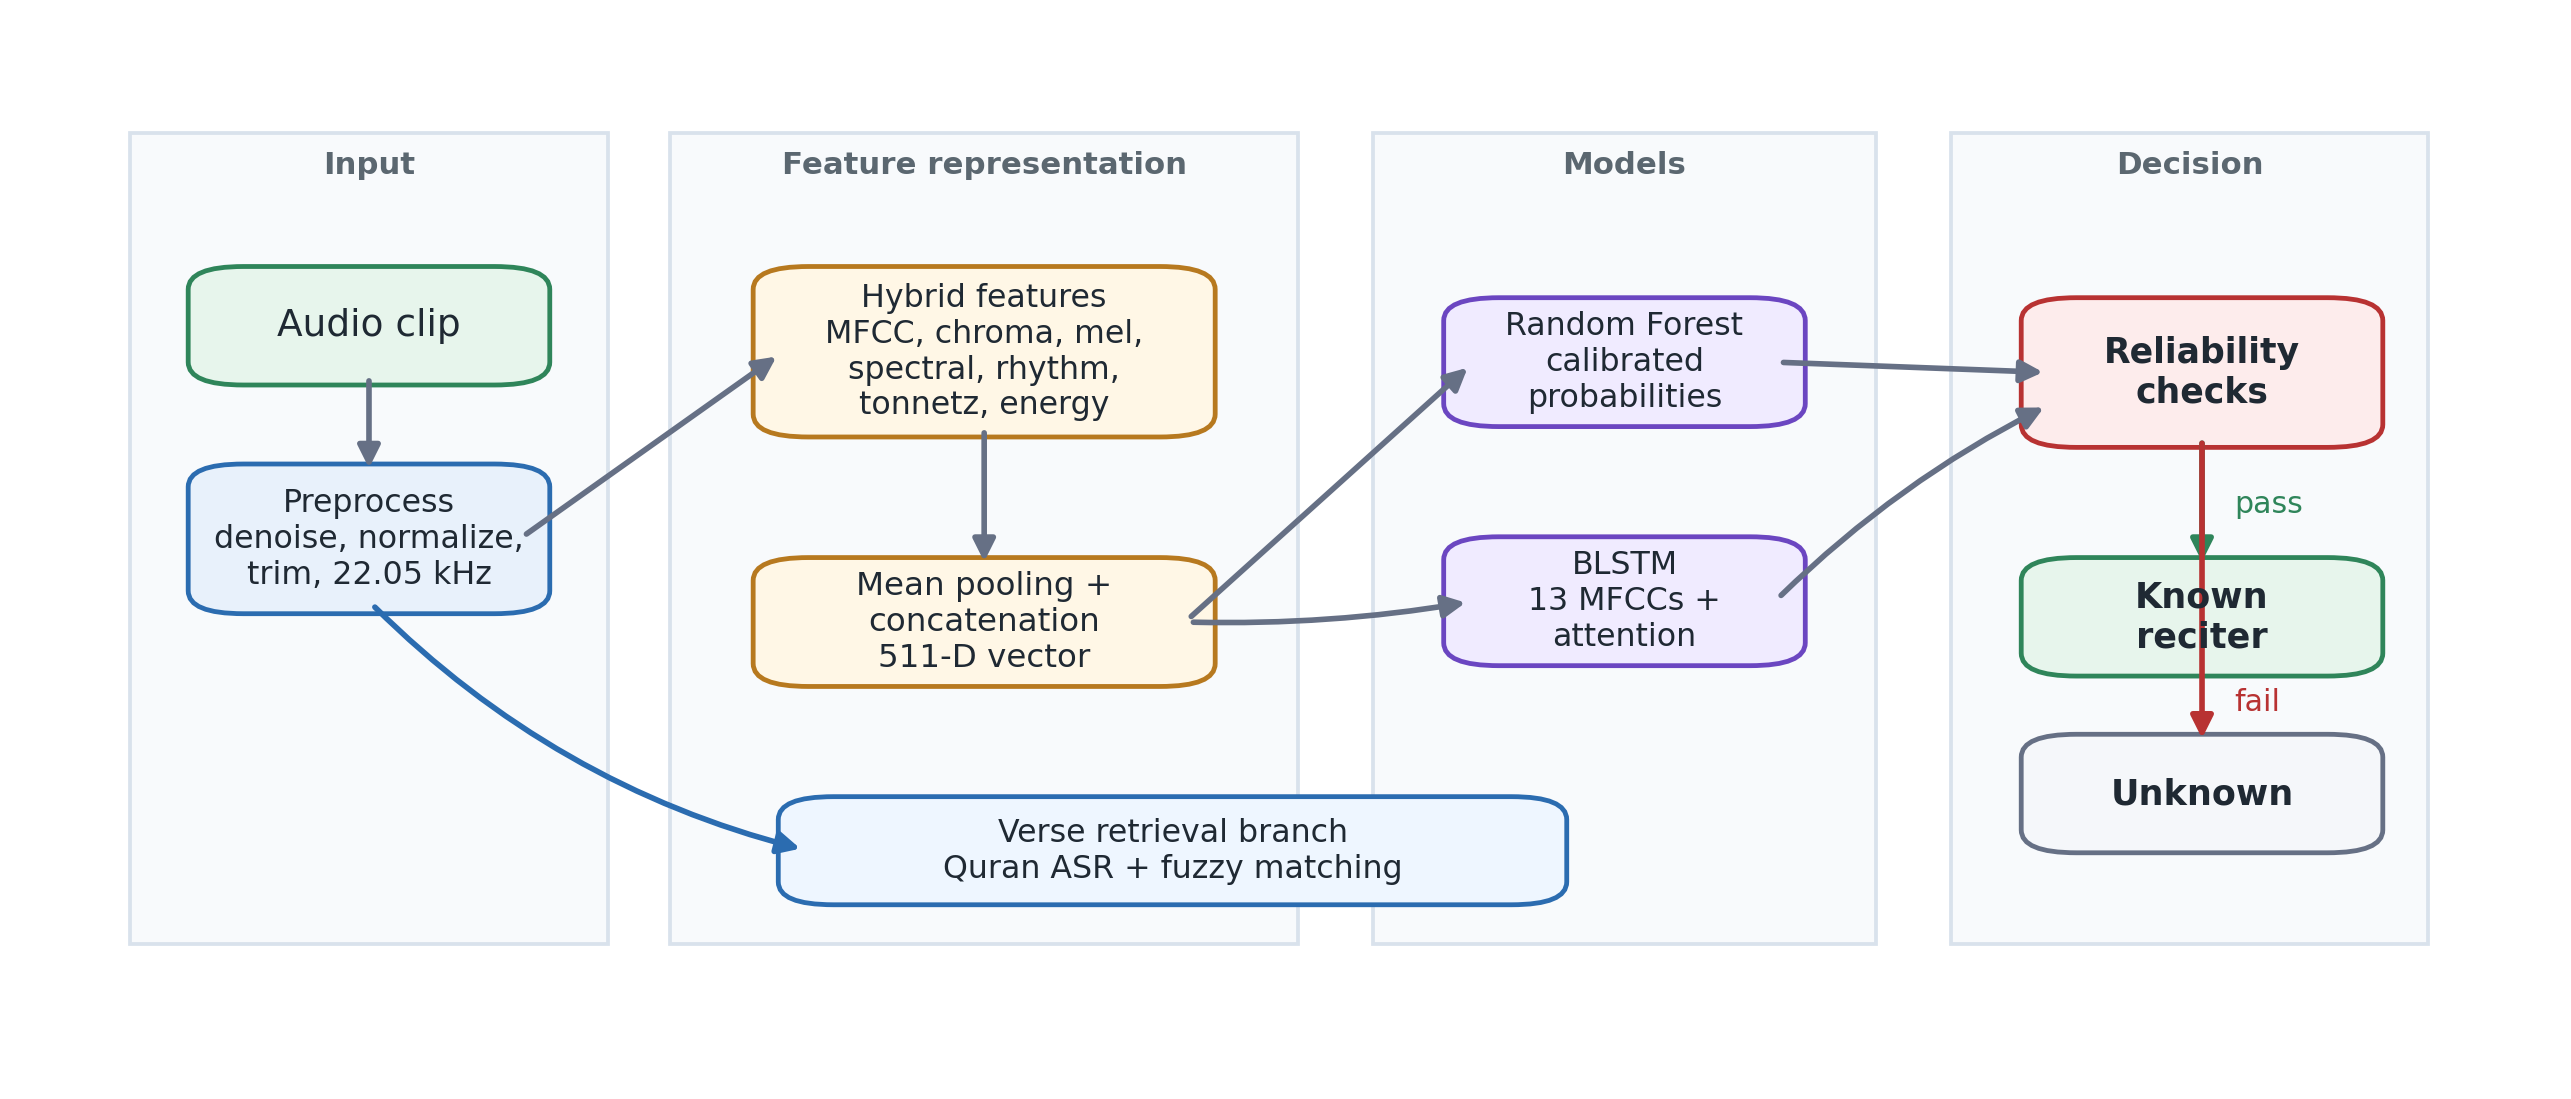
\includegraphics[width=0.82\textwidth]{figure1.png}
\caption{Overall architecture of the proposed Qurr\={a} open-set reciter recognition framework.}
\label{figure1}
\end{figure*}

\subsection{Audio Preprocessing and Feature Extraction}

All audio recordings are standardized prior to feature extraction. Each audio sample is converted to mono and resampled to 22,050 Hz. Silence trimming and normalization are applied to reduce variability caused by recording conditions.

The system employs a hybrid acoustic feature extraction approach that combines multiple categories of audio descriptors:

\begin{itemize}
\item Mel-Frequency Cepstral Coefficients (MFCC)
\item Chroma-based features
\item Mel-spectrogram energy bands
\item Spectral features (contrast, rolloff, centroid)
\item Temporal rhythm features (tempogram)
\item Tonal features (tonnetz)
\item Energy-based features (RMS, zero-crossing rate)
\end{itemize}

All features are computed at frame level and aggregated using temporal mean pooling across the entire audio clip.

For the Random Forest classifier, the resulting feature representation forms a \textbf{fixed-length 511-dimensional vector}. This vector is obtained by concatenating all aggregated feature blocks into a single representation.

For the BLSTM model, only the first 13 MFCC coefficients are retained and organized into fixed-length temporal sequences of length 16.

The complete processing pipeline is illustrated in Fig.~\ref{figure2}.

% -----------------------------
% Figure 2
% -----------------------------
\begin{figure}[htbp]
\centering
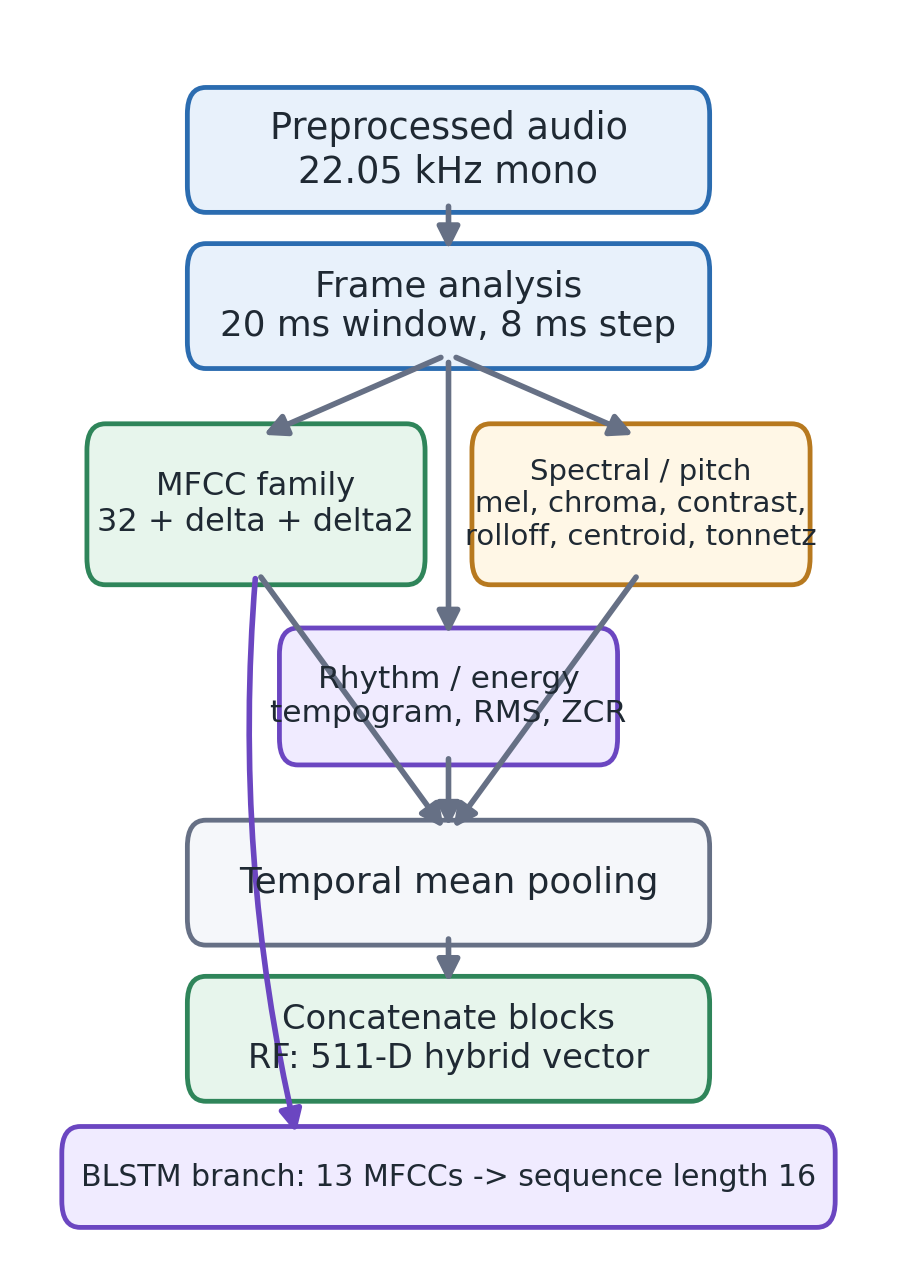
\includegraphics[width=\columnwidth]{figure2.png}
\caption{Hybrid acoustic feature extraction and processing pipeline.}
\label{figure2}
\end{figure}

\subsection{Random Forest Classifier}

The Random Forest classifier is used as a classical ensemble learning approach for reciter identification \cite{breiman}. The model consists of 100 decision trees with a maximum depth of 10. A fixed random seed is used for the data split and Random Forest training.

The classifier is trained using the full \textbf{511-dimensional feature vector}, which includes MFCC-based descriptors as well as spectral, chroma, rhythmic, and tonal features.

Probability calibration is applied to improve confidence estimation for open-set rejection. The model aggregates predictions from individual decision trees using majority voting.

This configuration enables the Random Forest model to operate as a robust classifier on high-dimensional acoustic feature representations without requiring temporal modeling.

\subsection{Bidirectional Long Short-Term Memory Classifier}

The BLSTM model is designed to capture temporal dependencies in Qur'anic recitation audio \cite{schuster}. The model receives a sequence of MFCC feature vectors derived from each audio clip.

The architecture consists of a single bidirectional LSTM layer with 64 hidden units in each direction. The output of the BLSTM layer is processed using an attention mechanism to emphasize relevant temporal segments of the audio sequence \cite{bahdanau}.

The final representation is passed through a fully connected classification layer to produce reciter predictions.

Training is performed using the AdamW optimizer with a learning rate of 0.0005 and batch size of 64. Early stopping and learning rate scheduling are applied to prevent overfitting and improve generalization.

\subsection{Reliability-Based Open-Set Recognition}

To enable open-set recognition, a reliability-based decision module is applied after classification. This module determines whether a prediction corresponds to a known reciter or should be rejected as unknown.

The reliability decision is based on four criteria:

\begin{enumerate}
\item Maximum prediction confidence
\item Secondary highest confidence score
\item Confidence margin between top two predictions
\item Distance-based similarity to class centroids
\end{enumerate}

A sample is accepted as a valid reciter prediction only if all reliability conditions are satisfied. Otherwise, the system assigns the label \textbf{Unknown}, indicating that the input does not belong to any known training class.

Let $p_1$ and $p_2$ denote the highest and second-highest predicted class probabilities, respectively. Let $d(x,c_1)$ denote the Euclidean distance between feature vector $x$ and the centroid of the predicted class $c_1$, and let $T(c_1)$ be the 95th-percentile intra-class distance threshold estimated from training data. The prediction is accepted only when
\begin{equation}
p_1 \geq 0.95 \ \land\ p_2 < 0.10 \ \land\ (p_1-p_2) \geq 0.80 \ \land\ \frac{d(x,c_1)}{T(c_1)} \leq 1.0.
\label{eq:reliability}
\end{equation}

This mechanism allows the system to operate in open-set conditions without explicitly training on an unknown class.

The decision workflow is illustrated in Fig.~\ref{figure3}.

% -----------------------------
% Figure 3
% -----------------------------
\begin{figure*}[t]
\centering
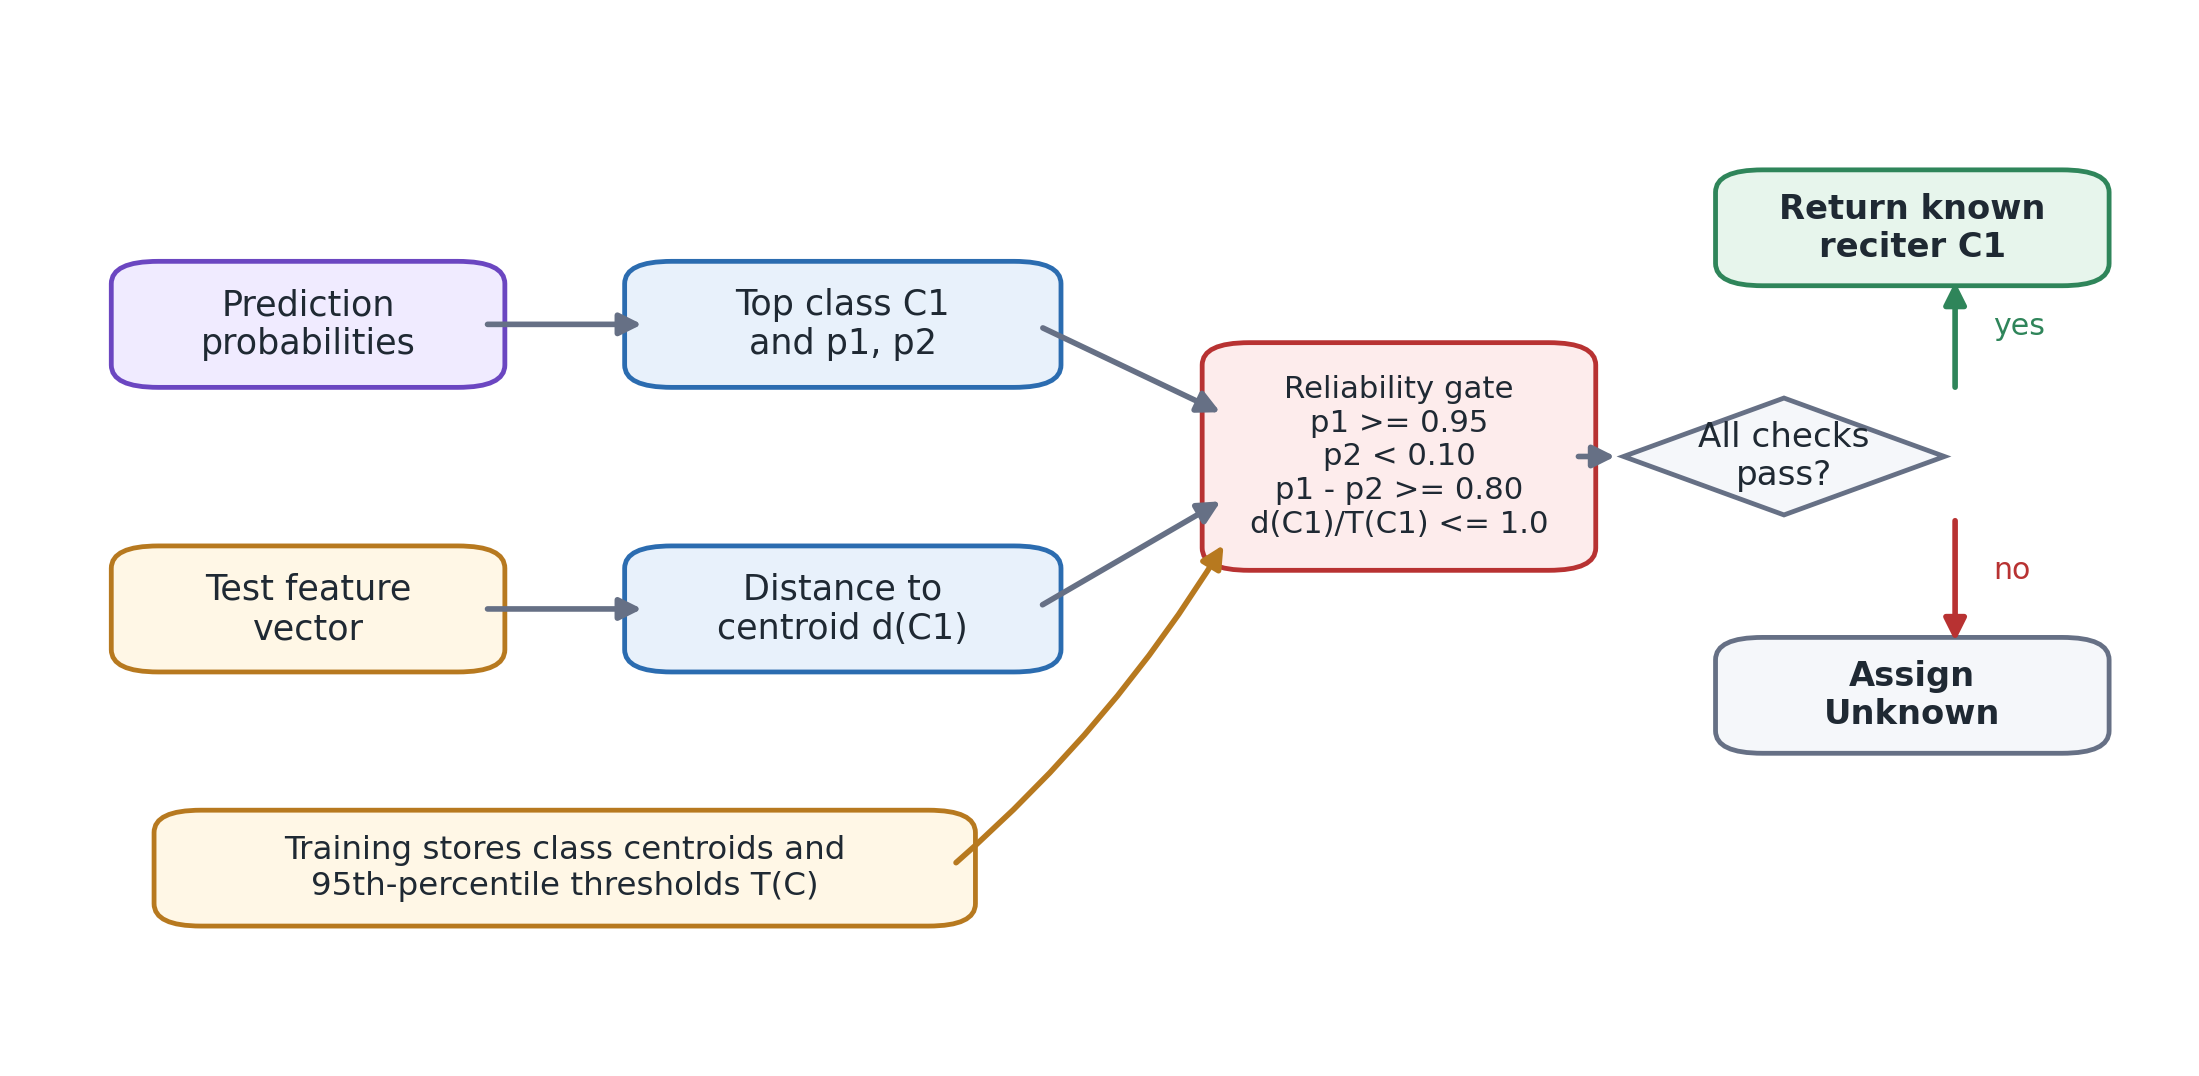
\includegraphics[width=0.72\textwidth]{figure3.png}
\caption{Reliability-based open-set recognition decision workflow.}
\label{figure3}
\end{figure*}

\subsection{Supporting Verse Retrieval Component}

In addition to reciter recognition, the framework includes a supporting Qur'anic verse retrieval component. This module is designed to map spoken recitation audio to corresponding Qur'anic verses.

The system uses the pretrained \texttt{tarteel-ai/whisper-base-ar-quran} speech-recognition model \cite{tarteelwhisper} to transcribe input audio into Arabic text. The resulting transcription is normalized and compared against a database of 6,236 Qur'anic verses using token-based similarity matching.

A fuzzy matching algorithm is used to identify the most likely corresponding verse(s) from the Qur'an database. This component is intended as a supplementary feature for educational applications and is not the primary focus of the current evaluation.

Due to limited availability of large-scale labeled test data, comprehensive benchmarking of this subsystem is left for future work.

\section{Experimental Setup}

\subsection{Dataset}

The experiments were conducted using a curated dataset of Qur'anic recitation audio recordings. The dataset consists of recordings from multiple Qur'anic reciters and is structured to evaluate both closed-set and open-set recognition performance.

The 2,535 recordings constitute the development corpus. A stratified 80/20 split produces a model-fitting partition of 2,028 recordings and a holdout partition of 507 recordings. The external test set is kept entirely separate from this development corpus. The resulting experimental partitions are:

\begin{itemize}
\item \textbf{Model-fitting set:} 2,028 audio recordings from 5 reciters
\item \textbf{Holdout set:} 507 audio recordings derived from a stratified 80/20 split of the 2,535-recording development corpus
\item \textbf{External test set:} 399 audio recordings from 7 reciters
\end{itemize}

The training reciters include: Abdulbasit Abdulsamad, Abdulrahman Alsudaes, Ahmad Al-Ajmy, Maher Al Meaqli, and Yasser Al-Dosari.

The external evaluation set includes both seen and unseen reciters, enabling open-set evaluation. Four reciters overlap with the training set, while three reciters are entirely unseen during training.

A key design feature of the dataset is \textbf{surah-level separation}. Training recordings are drawn from Surah 1 and Surahs 78--103, while external evaluation recordings are drawn exclusively from Surahs 104--114. This separation reduces content leakage and ensures that evaluation reflects reciter-specific generalization rather than memorization of Qur'anic content.

The corpus is a curated research collection assembled for this study rather than a standardized public benchmark. Because the redistribution status of individual recordings can vary by source, the audio files are not redistributed with the software. A manifest containing recording sources, reciter labels, surah identifiers, and the partition assignments should be made available to reviewers and future researchers.

% -----------------------------
% Table 1
% -----------------------------
\begin{table*}[t]
\centering
\caption{Dataset partitions used in the experimental evaluation.}
\label{table1}
\renewcommand{\arraystretch}{1.2}
\setlength{\tabcolsep}{6pt}
\resizebox{\textwidth}{!}{
\begin{tabular}{p{3cm} p{2.5cm} p{2cm} p{6.5cm}}
\toprule
\textbf{Partition} & \textbf{Recordings} & \textbf{Reciters} & \textbf{Details} \\
\midrule
Model-fitting set & 2,028 & 5 & Stratified 80\% of development corpus; Surah 1 and Surahs 78--103 \\
Holdout set & 507 & 5 & Stratified 20\% of development corpus \\
External test set & 399 & 7 & Surahs 104--114; includes seen and unseen reciters \\
\bottomrule
\end{tabular}
}
\end{table*}

\subsection{Data Preprocessing}

All audio recordings are standardized prior to feature extraction. Each audio sample is converted to mono and resampled to 22,050 Hz. The implementation uses the librosa audio-analysis library for feature extraction and signal operations \cite{librosa}.

Preprocessing includes:

\begin{itemize}
\item Silence trimming
\item Amplitude normalization
\item Noise reduction (basic filtering)
\item Duration validation to ensure consistency
\end{itemize}

After preprocessing, acoustic features are extracted using a unified feature extraction pipeline. These features are later used for both Random Forest and BLSTM models, although with different input representations.

\subsection{Model Training Configuration}

Two models are evaluated in this study: a Random Forest classifier and a Bidirectional LSTM network.

\subsubsection{Random Forest Configuration}

\begin{itemize}
\item Number of trees: 100
\item Maximum depth: 10
\item Random state: 42
\item Feature vector: 511-dimensional hybrid acoustic representation
\item Probability calibration applied for confidence estimation
\item 5-fold cross-validation on training data
\end{itemize}

\subsubsection{BLSTM Configuration}

\begin{itemize}
\item Input features: 13 MFCC coefficients
\item Sequence length: 16
\item Hidden units: 64 (bidirectional)
\item Attention mechanism applied to LSTM outputs
\item Optimizer: AdamW
\item Learning rate: 0.0005
\item Batch size: 64
\item Dropout: 0.5
\item Early stopping applied based on validation performance
\end{itemize}

Both models are trained on identical training partitions to ensure fair evaluation, although their input feature representations differ in dimensionality and structure.

% -----------------------------
% Table 2
% -----------------------------
\begin{table}[htbp]
\centering
\caption{Model training configurations for Random Forest and BLSTM classifiers.}
\label{table2}
\renewcommand{\arraystretch}{1.2}
\setlength{\tabcolsep}{4pt}
\resizebox{\columnwidth}{!}{
\begin{tabular}{p{1.4cm} p{2.8cm} p{2.8cm}}
\toprule
\textbf{Parameter} & \textbf{Random Forest} & \textbf{BLSTM} \\
\midrule
Input features & 511-dim hybrid vector & 13 MFCCs (seq. len. 16) \\
Architecture & 100 trees, depth 10 & BiLSTM (64 units) + attention \\
Optimizer & --- & AdamW (lr = 0.0005) \\
Batch size & --- & 64 \\
Regularization & Probability calibration & Dropout 0.5, early stopping \\
Random seed & 42 & 42 \\
\bottomrule
\end{tabular}
}
\end{table}

\subsection{Evaluation Protocol}

The evaluation is conducted using a multi-level protocol designed to assess both closed-set and open-set recognition performance.

The evaluation consists of four stages:

\begin{enumerate}
\item \textbf{Holdout Evaluation:} A stratified 20\% subset of the training dataset is used to evaluate model performance on unseen samples from known reciters.
\item \textbf{Closed-Set External Evaluation:} Evaluation is performed on 228 recordings from known reciters reciting previously unseen surahs (Surahs 104--114).
\item \textbf{Open-Set Evaluation:} Evaluation is performed on 171 recordings from unseen reciters not included in the training dataset.
\item \textbf{Combined External Evaluation:} A full evaluation on all 399 external test samples, combining both closed-set and open-set scenarios.
\end{enumerate}

For open-set evaluation, a reliability-based rejection mechanism is applied to determine whether a prediction should be accepted or labeled as unknown.

\subsection{Evaluation Metrics}

The following evaluation metrics are used to assess system performance:

\begin{itemize}
\item Accuracy
\item Precision
\item Recall
\item F1-score
\item Macro-averaged F1-score
\item False Positive Rate (for open-set evaluation)
\item Reject Accuracy (correct identification of unknown reciters)
\end{itemize}

For open-set evaluation, a prediction is considered correct if an unseen reciter is correctly rejected as \textbf{Unknown}.

\subsection{Experimental Reproducibility}

To ensure reproducibility, all experiments are conducted using fixed random seeds and consistent preprocessing configurations.

Key reproducibility settings include:

\begin{itemize}
\item Random seed: 42 (for Random Forest and dataset splitting)
\item Fixed preprocessing pipeline for all audio samples
\item Consistent feature extraction using librosa-based pipeline
\item Standardized sampling rate (22,050 Hz)
\item Fixed dataset partitions for training, holdout, and external evaluation
\end{itemize}

All trained models and evaluation outputs are stored with versioned identifiers to ensure traceability across experiments.

The dataset splits, model configurations, and evaluation scripts are fully deterministic, allowing experiments to be reproduced under identical conditions.

\section{Results and Discussion}
\fontsize{11}{13}\selectfont

\subsection{Holdout Evaluation}

The holdout evaluation was conducted using a stratified 20\% split of the training dataset, consisting of 507 audio recordings. This evaluation measures the performance of both models on unseen samples from known reciters.

The Random Forest classifier achieved an accuracy of \textbf{99.61\%}, while the BLSTM model achieved an accuracy of \textbf{99.01\%}. Both models demonstrated strong performance, indicating that the learned representations generalize well to unseen samples within the same distribution.

The high performance on the holdout set suggests that both models are capable of effectively capturing discriminative acoustic patterns associated with individual reciters.

\subsection{Closed-Set External Evaluation}

The closed-set external evaluation consists of 228 recordings from known training reciters reciting previously unseen surahs (Surahs 104--114).

In this setting, the Random Forest model achieved \textbf{100.0\% accuracy} with a Macro F1-score of \textbf{1.000}, indicating perfect classification performance under closed-set conditions.

The BLSTM model achieved \textbf{97.81\% accuracy}, with a Macro F1-score of \textbf{0.978}, showing a small degradation compared to the Random Forest model.

These results indicate that both models generalize well to unseen Qur'anic content, with Random Forest exhibiting slightly stronger robustness in this evaluation setting.

\subsection{Open-Set Rejection Performance}

The open-set evaluation consists of 171 recordings from unseen reciters not present in the training dataset.

The Random Forest model achieved a rejection accuracy of \textbf{97.66\%}, correctly identifying unseen reciters as unknown in the majority of cases. The BLSTM model achieved a rejection accuracy of \textbf{87.13\%}, indicating a higher tendency to misclassify unseen reciters as known classes.

These results demonstrate the effectiveness of the reliability-based rejection mechanism, particularly when combined with the Random Forest classifier.

\subsection{Overall External Evaluation}

The overall external evaluation combines both closed-set and open-set scenarios, totaling 399 recordings.

The Random Forest model achieved an overall accuracy of \textbf{95.24\%}, while the BLSTM model achieved \textbf{88.97\%}.

These results reflect the combined performance of classification accuracy on known reciters and rejection capability for unseen reciters. The Random Forest model consistently outperformed the BLSTM model across all evaluation categories.

% -----------------------------
% Table 3
% -----------------------------
\begin{table*}[t]
\centering
\caption{Summary of evaluation results across all experimental settings.}
\label{table3}
\renewcommand{\arraystretch}{1.2}
\setlength{\tabcolsep}{6pt}
\resizebox{\textwidth}{!}{
\begin{tabular}{p{4.5cm} p{2.5cm} p{2.5cm} p{2.5cm} p{2.5cm}}
\toprule
\textbf{Evaluation Setting} & \textbf{Samples} & \textbf{RF Result} & \textbf{BLSTM Result} & \textbf{Metric} \\
\midrule
Holdout evaluation & 507 & 99.61\% & 99.01\% & Accuracy \\
Closed-set external evaluation & 228 & 100.0\% (F1: 1.000) & 97.81\% (F1: 0.978) & Accuracy / Macro F1 \\
Open-set rejection & 171 & 97.66\% & 87.13\% & Rejection accuracy \\
Overall external evaluation & 399 & 95.24\% & 88.97\% & Accuracy \\
\bottomrule
\end{tabular}
}
\end{table*}

\subsection{Confusion Matrix Analysis}

The confusion matrices provide additional insight into model performance across reciters.

For the Random Forest model, the confusion matrix shows near-perfect diagonal dominance, indicating minimal misclassification across all reciter classes.

The BLSTM model shows a small number of misclassifications, primarily involving confusion between similar reciter voice characteristics, particularly for Yasser Al-Dosari.

In both models, errors are more prominent in boundary cases where acoustic similarities between reciters are higher.

Figures~\ref{figure4} and~\ref{figure5} present the confusion matrices for Random Forest and BLSTM models respectively.

% -----------------------------
% Figure 4
% -----------------------------
\begin{figure}[htbp]
\centering
\includegraphics[width=\columnwidth]{figure4.png}
\caption{Confusion matrix for the Random Forest classifier.}
\label{figure4}
\end{figure}

% -----------------------------
% Figure 5
% -----------------------------
\begin{figure}[htbp]
\centering
\includegraphics[width=\columnwidth]{figure5.png}
\caption{Confusion matrix for the BLSTM classifier.}
\label{figure5}
\end{figure}

\subsection{Discussion}

\subsubsection{Random Forest versus BLSTM}

The Random Forest classifier consistently outperforms the BLSTM model across all evaluation settings, including holdout, closed-set external evaluation, and open-set rejection.

This performance difference can be attributed to the fact that the Random Forest model utilizes a \textbf{full 511-dimensional hybrid acoustic feature representation}, incorporating MFCC, spectral, chroma, rhythmic, and tonal descriptors. In contrast, the BLSTM model operates only on a reduced subset of 13 MFCC coefficients arranged as temporal sequences.

This disparity in feature richness provides the Random Forest model with significantly more discriminative information, which likely contributes to its superior performance.

\subsubsection{Importance of Open-Set Evaluation}

Traditional closed-set evaluation assumes that all possible classes are known during training. However, real-world deployment of reciter recognition systems requires handling previously unseen reciters.

The open-set evaluation in this study demonstrates that incorporating a reliability-based rejection mechanism significantly improves practical usability. The Random Forest model, in particular, demonstrates strong rejection capability with a low false positive rate.

This highlights the importance of evaluating recognition systems under realistic open-set conditions rather than relying solely on closed-set accuracy.

\subsubsection{Supporting Verse Retrieval Component}

In addition to reciter recognition, the system includes a supporting verse retrieval component based on speech-to-text transcription using a pretrained Arabic Qur'anic speech recognition model.

Although this component is not the primary focus of the evaluation, it demonstrates the potential of integrating recitation understanding with verse-level retrieval, enabling educational applications such as recitation verification and learning assistance.

\subsubsection{Threats to Validity}

Several limitations should be considered when interpreting the results of this study.

First, the dataset is limited to a fixed set of reciters and surahs, which may not fully represent the diversity of global Qur'anic recitation styles.

Second, although open-set evaluation is included, the reliability thresholds used for rejection are fixed and not dynamically learned, which may affect generalization in different environments.

Third, the BLSTM model uses a reduced feature representation compared to the Random Forest model, which may introduce an imbalance in model capacity rather than purely architectural differences.

Finally, the verse retrieval component has not been evaluated on a large-scale benchmark dataset, and its performance remains exploratory.

\section{Conclusion}
\fontsize{11}{13}\selectfont

This paper presented Qurr\={a}, an open-set Qur'anic reciter recognition framework designed to identify known reciters while rejecting previously unseen reciters. The proposed system integrates a hybrid acoustic feature representation with a reliability-based classification mechanism and evaluates two machine learning approaches: Random Forest and Bidirectional Long Short-Term Memory (BLSTM) networks.

The experimental results demonstrate that the Random Forest classifier consistently outperforms the BLSTM model across all evaluation settings. On the holdout dataset, both models achieved high accuracy, with Random Forest reaching 99.61\% and BLSTM achieving 99.01\%. On the closed-set external evaluation involving unseen Qur'anic surahs, Random Forest achieved perfect classification accuracy of 100\%, while BLSTM achieved 97.81\%. In the open-set evaluation involving previously unseen reciters, Random Forest achieved a rejection accuracy of 97.66\%, significantly outperforming BLSTM, which achieved 87.13\%. Overall external evaluation results further confirm the superiority of Random Forest, with accuracies of 95.24\% and 88.97\% for Random Forest and BLSTM respectively.

A key contribution of this work is the introduction of a hybrid acoustic feature representation combining MFCC, spectral, chroma, rhythmic, and tonal descriptors. This representation enables the Random Forest classifier to leverage a rich 511-dimensional feature space, while the BLSTM model operates on a reduced MFCC-based sequential representation. Additionally, the proposed reliability-based rejection mechanism enables effective open-set recognition without requiring explicit training on unknown classes.

The study also introduces a structured evaluation protocol that separates training and testing data by Qur'anic surah content and incorporates both closed-set and open-set scenarios. This provides a more realistic assessment of model generalization compared to traditional closed-set evaluation approaches.

Despite the strong performance achieved, several directions for future work remain. First, the open-set rejection mechanism relies on manually defined reliability thresholds, which could be improved through adaptive or learned calibration strategies. Second, the BLSTM model could benefit from access to the full hybrid feature representation to enable a more balanced comparison with the Random Forest classifier. Third, expanding the dataset to include a larger and more diverse set of reciters and recitation styles would improve generalization and robustness. Finally, further investigation into transformer-based architectures may provide additional improvements for sequential modeling of Qur'anic recitation audio.

Overall, the results demonstrate that carefully engineered acoustic feature representations combined with classical ensemble learning methods remain highly effective for Qur'anic reciter recognition, particularly in open-set scenarios where system reliability and rejection capability are critical.

\balance
\fontsize{11}{13}\selectfont
\printbibliography

\end{document}
